
\begin{figure}[H]    
    \centering
    \begin{minipage}{.25\textwidth}
        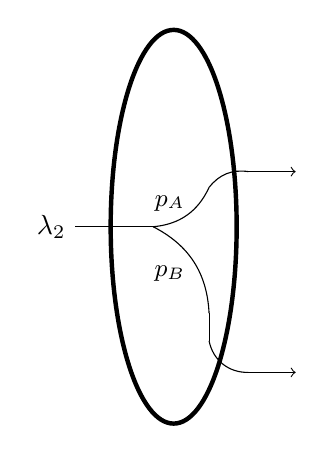
\begin{tikzpicture}
            \draw[ultra thick] (0.75,2) ellipse (0.8cm and 2.5cm);
            % \draw (0,0) -- ++(1.5cm,0) -- ++(0,4cm) -- ++(-1.5cm,0) -- ++ (0, -4cm);
            \draw[-] (0.5, 2) -- ++(-1, 0) node[left] {\(\lambda_2\)};
            
            % p_A line
            \path (0.49, 2) edge [bend right=30] (1.2, 2.5);
            \path (1.2, 2.5) edge [bend left=30] (1.7, 2.7);
            \draw[->] (1.7, 2.7) -- ++(0.6, 0.);
            
            % p_B
            \path (0.49, 2) edge [bend left=30] (1.2, 0.9);
            \draw[-] (1.2, 0.9) -- (1.2, 0.55);
            \path (1.2, 0.55) edge [bend right=40] (1.7, 0.15);
            \draw[->] (1.7, 0.15) -- ++(0.6, 0.);

            \node at (0.7, 2.3) {\small{\( p_A \)}};
            \node at (0.7, 1.4) {\small{\( p_B \)}};
        \end{tikzpicture}
    \end{minipage}
    \begin{minipage}{.55\textwidth}
        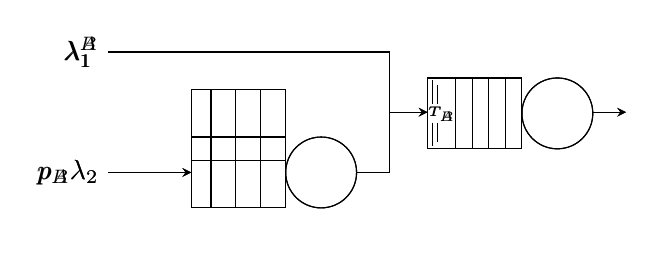
\begin{tikzpicture}[>=stealth, scale=0.6] %arrow type
            % Difference between the two queue diagrams
            \tikzmath{
                let \diff = -4.5cm;
            }

            % the rectangle with vertical lines (Queue 1)
            \draw (0,0) -- ++(2cm,0) -- ++(0,-1.5cm) -- ++(-2cm,0);
            \foreach \i in {1,...,3, 3.8}
            \draw (2cm-\i*15pt,0) -- +(0,-1.5cm);
            
            % the circle (Queue 1)
            \draw (2.75,-0.75cm) circle [radius=0.75cm];
    
            % the rectangle with vertical lines (Queue 2)
            \draw (5,1.25) -- ++(2cm,0) -- ++(0,-1.5cm) -- ++(-2cm,0);
            \foreach \i in {1,...,4, 5.7}
            \draw (7cm-\i*10pt,1.25) -- +(0,-1.5cm);

            % The two vertical lines at the start of Queue 2 
            \draw (7cm-54pt, 1.2cm) -- +(0,-0.5cm);
            \draw (7cm-54pt, 0.3cm) -- +(0,-0.5cm);        
            \draw (7cm-51pt, 1.1cm) -- +(0,-0.4cm);
            \draw (7cm-51pt, 0.3cm) -- +(0,-0.4cm);
    
            % The label between the lines for T
            \node[anchor=north] at (5.3, 0.84) {\tiny{\( T_A \)}};

            % the circle (Queue 2)
            \draw (7.75,0.5) circle [radius=0.75cm];
    
            % the arrows and labels (Queue 1+2)
            \draw[->] (8.5,0.525) -- +(20pt,0);
            \node[align=center] at (1cm,-2cm) {};
            \node[align=center] at (6cm,-0.75cm) {};
            
            % Ambulance lines
            \draw[<-] (0,-0.75) -- +(-50pt,0) node[left] {\( p_A \lambda_2 \)};
            \draw[-] (3.5,-0.75) -- +(20pt,0);
            \draw (4.2, 0.525) -- (4.2, -0.75);

            % Others lines
            \draw (4.2, 1.8) -- +(-169.5pt,0) node[left] {\( \lambda_1^A \)};
            \draw (4.2, 1.8) -- (4.2, 0.525);
            \draw[->] (4.2, 0.525) -- (5, 0.525);

            % the rectangle with vertical rules (Queue 1)
            \draw (0, \diff) -- ++(2cm,0) -- ++(0,-1.5cm) -- ++(-2cm,0);
            \foreach \i in {1,...,3, 3.8}
            \draw (2cm-\i*15pt,\diff) -- +(0,-1.5cm);
            
            % the circle (Queue 1)
            \draw (2.75,\diff - 0.75cm) circle [radius=0.75cm];
    
            % the rectangle with vertical rules (Queue 2)
            \draw (5,\diff + 1.25cm) -- ++(2cm,0) -- ++(0,-1.5cm) -- ++(-2cm,0);
            \foreach \i in {1,...,4, 5.7}
            \draw (7cm-\i*10pt,\diff + 1.25cm) -- +(0,-1.5cm);

            % The two vertical lines at the start of Queue 2 
            \draw (7cm-54pt,\diff + 1.2cm) -- +(0,-0.5cm);
            \draw (7cm-54pt,\diff + 0.3cm) -- +(0,-0.5cm);        
            \draw (7cm-51pt,\diff + 1.1cm) -- +(0,-0.4cm);
            \draw (7cm-51pt,\diff + 0.3cm) -- +(0,-0.4cm);

            % The label between the lines for T
            \node[anchor=north] at (5.3, \diff + 0.84cm) {\tiny{\( T_B \)}};

            % the circle (Queue 2)
            \draw (7.75,\diff + 0.5cm) circle [radius=0.75cm];
    
            % the arrows and labels (Queue 1+2)
            \draw[->] (8.5, \diff + 0.525cm) -- +(20pt,0);
            \node[align=center] at (1cm,\diff-2cm) {};
            \node[align=center] at (6cm,\diff-0.75cm) {};
            
            % Ambulance lines
            \draw[<-] (0, \diff - 0.75cm) -- +(-50pt,0) node[left] {\( p_B \lambda_2 \)};
            \draw[-] (3.5, \diff - 0.75cm) -- +(20pt,0);
            \draw (4.2, \diff + 0.525cm) -- (4.2, \diff - 0.75cm);

            % Others lines
            \draw (4.2, \diff + 1.8cm) -- +(-169.5pt,0) node[left] {\( \lambda_1^B \)};
            \draw (4.2, \diff + 1.8cm) -- (4.2, \diff + 0.525);
            \draw[->] (4.2, \diff + 0.525cm) -- (5, \diff + 0.525cm);
        \end{tikzpicture}
    \end{minipage}
    \caption{Queue}
    \label{fig:diagram_of_game_theoretic_model}
\end{figure}